% interactcadsample.tex
% v1.03 - April 2017

\documentclass[]{interact}

\usepackage{epstopdf}% To incorporate .eps illustrations using PDFLaTeX, etc.
\usepackage{subfigure}% Support for small, `sub' figures and tables
%\usepackage[nolists,tablesfirst]{endfloat}% To `separate' figures and tables from text if required

\usepackage{natbib}% Citation support using natbib.sty
\bibpunct[, ]{(}{)}{;}{a}{}{,}% Citation support using natbib.sty
\renewcommand\bibfont{\fontsize{10}{12}\selectfont}% Bibliography support using natbib.sty

\theoremstyle{plain}% Theorem-like structures provided by amsthm.sty
\newtheorem{theorem}{Theorem}[section]
\newtheorem{lemma}[theorem]{Lemma}
\newtheorem{corollary}[theorem]{Corollary}
\newtheorem{proposition}[theorem]{Proposition}

\theoremstyle{definition}
\newtheorem{definition}[theorem]{Definition}
\newtheorem{example}[theorem]{Example}

\theoremstyle{remark}
\newtheorem{remark}{Remark}
\newtheorem{notation}{Notation}

% see https://stackoverflow.com/a/47122900

% Pandoc citation processing

\usepackage{hyperref}
\usepackage[utf8]{inputenc}
\def\tightlist{}


\begin{document}

\articletype{ARTICLE TEMPLATE}

\title{Why shouldn't you use numerical tests to diagnose the linear
regression models?}


\author{\name{Weihao Li$^{a}$, Dianne Cook$^{a}$, Emi Tanaka$^{a}$}
\affil{$^{a}$Department of Econometrics and Business Statistics, Monash
University, Clayton, VIC, Australia}
}

\thanks{CONTACT Weihao
Li. Email: \href{mailto:weihao.li@monash.edu}{\nolinkurl{weihao.li@monash.edu}}, Dianne
Cook. Email: \href{mailto:dicook@monash.edu}{\nolinkurl{dicook@monash.edu}}, Emi
Tanaka. Email: \href{mailto:emi.tanaka@monash.edu}{\nolinkurl{emi.tanaka@monash.edu}}}

\maketitle

\begin{abstract}
Abstract to fill.
\end{abstract}

\begin{keywords}
visual inference; regression diagnostics;
\end{keywords}

\hypertarget{introduction}{%
\section{Introduction}\label{introduction}}

Regression analysis is a field of study with at least a hundred years of
history, and regression diagnostics is one of the essential steps in
regression analysis. The diagnostic procedure conventionally involves
evaluating the fitness of the proposed model, detecting the presence of
influential observations and outliers, checking the validity of model
assumptions and many more. In terms of diagnostic techniques, data
plots, hypothesis testing, and summary statistics are vital tools for a
systematic and detailed examination of the regression model
\citep{mansfield1987diagnostic}.

Many of those regression diagnostic methods and procedures are mature
and well-established in books first published in the twentieth century,
such as \citet{draper_applied_2014},
\citet{montgomery_introduction_2012}, \citet{belsley_regression_1980},
\citet{cook_applied_1999} and \citet{cook1982residuals}. Regardless of
the level of difficulty, one will find the importance and usefulness of
diagnostic plots being emphasized in those books repeatedly. Checking
diagnostic plots is also the recommended starting point for validating
model assumptions such as normality, homoscedasticity and linearity
\citep{anscombe_examination_1963}.

\hypertarget{diagnostic-plots}{%
\subsection{Diagnostic plots}\label{diagnostic-plots}}

Graphical summaries in which residuals are plotted against fitted values
or other functions of the predictor variables that are approximately
orthogonal to residuals are referred to as standard residual plots in
\citet{cook1982residuals}. As suggested by \citet{cook1982residuals},
these kinds of diagnostic plots are commonly used to identify patterns
that are indicative of nonconstant error variance or non-linearity. Raw
residuals and studentized residuals are the two most frequently used
residuals in standard residual plots. The debt on which type of
residuals should be used is always present. While raw residuals are the
most common computer regression software package output, by applying a
scaling factor, the ability to reveal nonconstant error variance in
standard residual plots will often be enhanced by studentized residuals
in small sample size \citep{gunst2018regression}. As a two-dimensional
representation of a model in a \(p\)-dimensional space, standard
residual plots project data points onto the variable of the horizontal
axis, which is a vector in \(p\)-dimensional space. Observations with
the same projection will be treated as equivalent as they have the same
abscissa. Therefore, standard residual plots are often useful in
revealing model inadequacies in the direction of the variable of the
horizontal axis but could be inadequate for detecting patterns in other
directions, especially in those perpendicular to the variable of the
horizontal axis. Hence, in practice, multiple standard residual plots
with different horizontal axes will be examined
\citep{cook1982residuals}. Overlapping data points is a general issue in
scatter plots not limited to standard residual plots, which often makes
plots difficult to interpret because visual patterns are concealed.
Thus, for a relatively large sample size, \citet{cleveland1975graphical}
suggests the use of robust moving statistics as reference lines to give
aid to the eye in seeing patterns, which nowadays, are usually replaced
with a spline or local polynomial regression line.

Other types of data plots that are often used in regression diagnostics
include partial residual plots and probability plots. Partial residual
plots are useful supplements to standard residual plots as they provide
additional information on the extent of the non-linearity. Probability
plots can be used to compare the sampling distribution of the residuals
to the normal distribution for assessing the normality assumptions.

\hypertarget{hypothesis-testing}{%
\subsection{Hypothesis testing}\label{hypothesis-testing}}

In addition to diagnostic plots, analysts may perform formal hypothesis
testing for detecting model defects. Depends on the alternative
hypothesis that being focused on, variety of tests can be applied. For
example, the presence of heteroskedasticity can usually be tested by
applying the White test \citep{white_heteroskedasticity-consistent_1980}
or the Breusch-Pagan test \citep{breusch_simple_1979}, which both
derived from the Lagrange multiplier test (ref here) principle and rely
on the asymptotic properties of the null distribution. For testing
non-linearity, one may apply the F-test (ref here) to examine the
significance of certain polynomial and non-linear forms of the
regressors, or the significance of proxy variables as in the Ramsey
Regression Equation Specification Error Test (RESET)
\citep{ramsey_tests_1969}.

As discussed in \citet{cook1982residuals}, most residual-based tests for
a particular type of departure from model assumptions are sensitive to
other types of departures. It is likely the null hypothesis is correctly
rejected but for the wrong reason, which is also known as the ``Type III
error''. Additionally, outliers will often incorrectly trigger the
rejection of the null hypothesis despite the residuals being
well-behaved \citep{cook_applied_1999}. This can be largely avoided in
diagnostic plots as experienced analysts can evaluate the acceptability
of assumptions flexibly, even in the presence of outliers.
\citet{montgomery_introduction_2012} stated that based on their
experience, statistical tests are not widely used in regression
diagnostics. The same or even larger amount of information can be
provided by diagnostic plots than the corresponding tests in most
empirical studies. Not to mention, it is almost impossible to have an
exactly correctly specified model in reality. There is a well-known
aphorism in statistics stated by George Box - ``All models are wrong,
but some are useful''. This indicates proper hypothesis tests will
always reject the null hypothesis as long as the sample size is large
enough. The outcome ``Not reject'' can be interpreted as either ``effect
size is small'' or ``sample size is small''. The outcome ``reject''
still doesn't inform us whether and how much the model defects are of
actual consequence to the inference and prediction. But still, the
effectiveness of statistical tests shall not be disrespected.
Statistical tests have a chance to provide analysts with unique
information. There are situations where no suitable diagnostic plots can
be found for a particular violation of the assumptions, or excessive
diagnostic plots need to be checked. One will have no choice but to rely
on statistical tests if there are any. A good regression diagnostic
practice should be a balanced combination of both methods.

\hypertarget{visual-inference}{%
\subsection{Visual inference}\label{visual-inference}}

However, unlike hypothesis testing built upon rigorous statistical
procedures, reading diagnostic plots relies on graphical perception -
human's ability to interpret and decode the information embedded in the
graph \citep{cleveland_graphical_1984}, which is to some extent
subjective. Further, visual discovery suffers from its unsecured and
unconfirmed nature where the degree of the presence of the visual
features typically can not be measured quantitatively and objectively,
which may lead to over or under-interpretations of the data. One such
example is finding an over-interpretation of the separation between gene
groups in a two-dimensional projection from a linear discriminant
analysis when in fact there are no differences in the expression levels
between the gene groups and separation is not an uncommon occurrence
\citep{roy_chowdhury_using_2015}.

Visual inference was first introduced in a 1999 Joint Statistical
Meetings (JSM) talk with the title ``Inference for Data Visualization''
by \citet{buja_inference_1999} as an idea to address the issue of valid
inference for visual discoveries of data plots
\citep{gelman_exploratory_2004}. Later, in the Bayesian context, data
plots was systematically considered as model diagnostics by taking
advantage of the data simulated from the assumed statistical models
\citep{gelman_bayesian_2003, gelman_exploratory_2004}.

It was surprising that the essential components of visual inference had
actually been established in \citet{buja_inference_1999}, but it was not
until 10 years later that \citet{buja_statistical_2009} formalized it as
an inferential framework to extend confirmatory statistics to visual
discoveries. This framework redefines the test statistics, tests, null
distribution, significance levels and \(p\)-value for visual discovery
modelled on the confirmatory statistical testing. Figure
@ref(fig:parallelism) outlines the parallelism between conventional
tests and visual discovery.

\begin{figure}
\centering
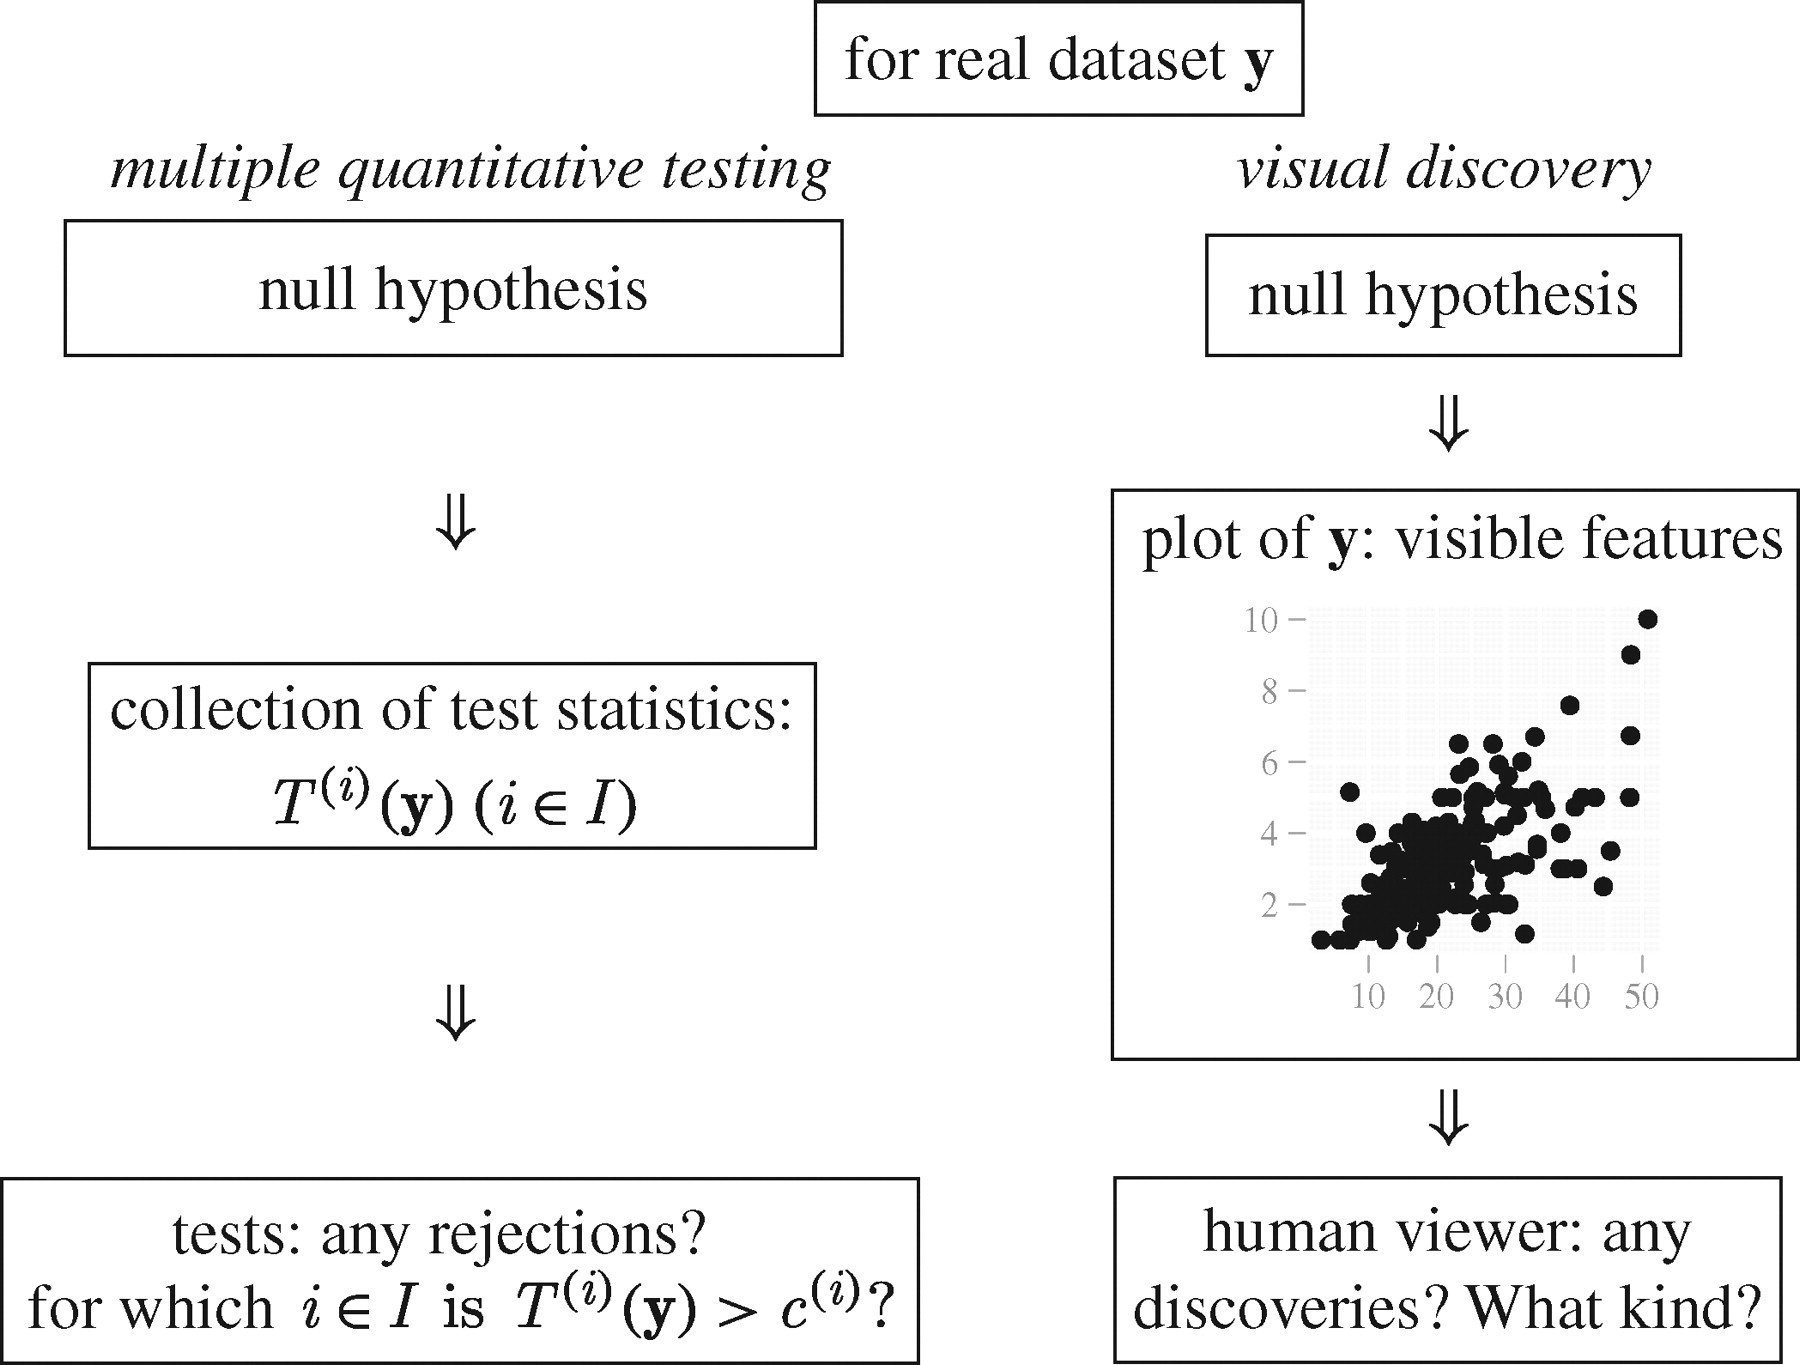
\includegraphics[width=4.6875in,height=3.55208in]{figures/rsta2009012001.jpg}
\caption{(ref:parallelism) \label{fig:parallelism}}
\end{figure}

(ref:parallelism) Parallelism between multiple quantitative testing and
visual discovery \citep{buja_statistical_2009}. Visible features in a
plot are viewed as a collection of test statistics
\(T^{(i)}(\boldsymbol{\mathrm{y}})~(i \in I)\), and any visual
discoveries that are inconsistent with the null hypothesis are treated
as evidence against the null. For regression diagnostics, the null
hypothesis would be the assumed model, and visual discoveries could be
any visual features in favour of any alternatives.

In visual inference, a collection of test statistics
\(T^{(i)}(\boldsymbol{\mathrm{y}})~(i \in I)\) is defined, where
\(\boldsymbol{\mathrm{y}}\) is the data and \(I\) is a set of all
possible visual features. \citet{buja_statistical_2009} described each
of the test statistics \(T^{(i)}(\boldsymbol{\mathrm{y}})\) as a
measurement of the degree of presence of a visual feature.
Alternatively, \citet{majumder_validation_2013} avoids the use of visual
features and defined the visual statistics \(T(.)\) as a mapping from a
dataset to a data plot. Both definitions of visual test statistics are
valid, but in the rest of the report the first definition will be used
as it covers some details needed by the following discussion. A visual
discovery is defined as a rejection of a null hypothesis, and the same
null hypothesis can be rejected by many different visual discoveries
\citep{buja_statistical_2009}. For regression diagnostics, the null
hypothesis would be the assumed model, while the visual discoveries
would be any findings that are inconsistent with the null hypothesis.
The same regression model can be rejected by many reasons with residual
plot, including non-linearity and heteroskedasticity as shown in Figure
@ref(fig:residual-plot-cubic-heter).

\begin{figure}
\centering
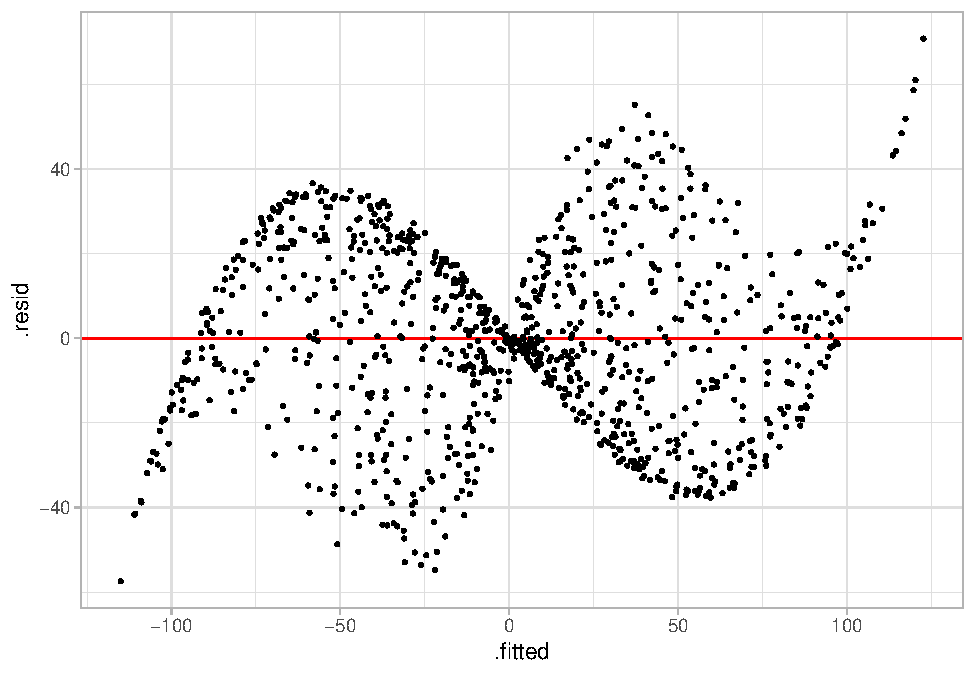
\includegraphics{paper_comparison_files/figure-latex/residual-plot-cubic-heter-1.pdf}
\caption{Residuals vs.~fitted values plot for a classical linear
regression model. The residuals are produced by fitting a two-predictor
multiple linear regression model with data generated from a cubic linear
model. From the residual plot, ``butterfly shape'' can be observed which
generally would be interpretd as evidence of heteroskedasticity.
Further, from the outline of the shape, nonlinear patterns exist. Both
visual discoveries are evidence against the null hypothesis, though
heteroskedasticity actually does not exist in the data generating
process.}
\end{figure}

\hypertarget{se:sampling-from-null}{%
\subsubsection{Sampling from the null
distribution}\label{se:sampling-from-null}}

The null distribution of plots refers to the infinite collection of
plots of null datasets sampled from \(H_0\). It is defined as the
analogue of the null distribution of test statistics in conventional
test \citep{buja_statistical_2009}. In practice, a finite number of
plots of null datasets could be generated, called null plots. In the
context of regression diagnostics, sampling data from \(H_0\) is
equivalent to sampling data from the assumed model. As
\citet{buja_statistical_2009} suggested, \(H_0\) is usually composited
by a collection of distributions controlled by nuisance parameters.
Since regression models can have various forms, there is no general
solution to this problem, but it sometimes can be reduced to so called
``reference distribution'' by applying one of the three methods: (i)
sampling from a conditional distribution given a minimal sufficient
statistic under \(H_0\), (ii) parametric bootstrap sampling with
nuisance parameters estimated under \(H_0\), and (iii) Bayesian
posterior predictive sampling.

The conditional distribution given a minimal sufficient statistic is the
best justified reference distribution among the three
\citep{buja_statistical_2009}. Suppose there exists a minimal sufficient
statistic \(\boldsymbol{S}(\boldsymbol{y})\) under the null hypothesis,
any null datasets \(\boldsymbol{y^{*}}\) should fulfil the condition
\(\boldsymbol{S}(\boldsymbol{y}) = \boldsymbol{s}\). Using the classical
normal linear regression model as example, the minimal sufficient
statistic is
\(\boldsymbol{S}(\boldsymbol{y}) = (\hat{\boldsymbol{\beta}}, \boldsymbol{e}'\boldsymbol{e})\),
where \(\hat{\boldsymbol{\beta}}\) are the coefficient estimators and
\(\boldsymbol{e}'\boldsymbol{e}\) is the residual sum of square.
Alternatively, the minimal sufficient statistic can be constructed as
\(\boldsymbol{S}(\boldsymbol{y}) = (\hat{\boldsymbol{y}}, ||\boldsymbol{e}||)\),
where \(\hat{\boldsymbol{y}}\) are the fitted values and
\(||\boldsymbol{e}||\) is the length of residuals, which is more
intuitive as suggested by \citet{buja_statistical_2009}. Since the
fitted values are held fixed, the variation can only occur in the
residual space. And because the length of residual is also held fixed,
residuals obtained from a null dataset has to be a random rotation of
\(\boldsymbol{e}\) in the residual space. With this property, null
residuals can be simulated by regressing \(N\) i.i.d standard normal
random draws on the regressors, then rescaling it by the ratio of
residual sum of square in two regressions.

\hypertarget{se:lineup}{%
\subsubsection{Lineup protocol}\label{se:lineup}}

With the simulation of null plots being provided, another aspect of
hypothesis testing that needs to be addressed is the control of false
positive rate or Type I error. Any visual statistic
\(T^{(i)}(\boldsymbol{\mathrm{y}})\) needs to pair with a critical value
\(c^{(i)}\) to form a hypothesis test. When a visual feature \(i\) is
discovered by the observer from a plot, the corresponding visual
statistic \(T^{(i)}(\boldsymbol{\mathrm{y}})\) may not be known as there
is no general agreement on the measurement of the degree of presence of
a visual feature. It is only the event that
\(T^{(i)}(\boldsymbol{\mathrm{y}}) > c^{(i)}\) is confirmed. Similarly,
if any visual discovery is found by the observer, we say, there exists
\(i \in I:~T^{(i)}(\boldsymbol{\mathrm{y}}) > c^{(i)}\)
\citep{buja_statistical_2009}.

Using the above definition, the family-wise Type I error can be
controlled if one can provide the collection of critical values
\(c^{(i)}~(i \in I)\) such that
\(P(\mathrm{there~exists~} i \in I: T^{(i)}(\boldsymbol{\mathrm{y}}) > c^{(i)}|\boldsymbol{\mathrm{y}}) \leq \alpha\),
where \(\alpha\) is the significance level. However, since the quantity
of \(T^{(i)}(\boldsymbol{\mathrm{y}})\) may not be known, such
collection of critical values can not be provided.

\citet{buja_statistical_2009} proposed the lineup protocol as a visual
test to calibrate the Type I error issue without the specification of
\(c^{(i)}~(i \in I)\). It is inspired by the ``police lineup'' or
``identity parade'' which is the act of asking the eyewitness to
identify criminal suspect from a group of irrelevant people. The
protocol consists of \(m\) randomly placed plots, where one plot is the
actual data plot, and the remaining \(m - 1\) plots have the identical
graphical production as the data plot except the data has been replaced
with data consistent with the null hypothesis. Then, an observer who
have not seen the actual data plot will be asked to point out the most
different plot from the lineup.

Under the null hypothesis, it is expected that the actual data plot
would have no distinguishable difference with the null plots, and the
probability of the observer correctly picks the actual data plot is
\(1/m\). If we reject the null hypothesis as the observer correctly
picks the actual data plot, then the Type I error of this test is
\(1/m\).

This provides us with an mechanism to control the Type I error, because
\(m\) - the number of plots in a lineup can be chosen. A larger value of
\(m\) will result in a smaller Type I error, but the limit to the value
of \(m\) depends on the number of plots a human is willing to view
\citep{buja_statistical_2009}. Typically, \(m\) will be set to \(20\)
which is equivalent to set \(\alpha = 0.05\), a general choice of
significance level for conventional testing among statisticians.

Further, if we involve \(K\) independent observers in a visual test, and
let \(X\) be a random variable denoting the number of observers
correctly picking the actual data plot. Then, under the null hypothesis
\(X \sim \mathrm{Binom}_{K,1/m}\), and therefore, the \(p\)-value of a
lineup of size \(m\) evaluated by \(K\) observer is given as
\begin{equation} \label{eq:pvaluesingle}
P(X \geq x) = \sum_{i=x}^{K}{{K}\choose{i}}\left(\frac{1}{m}\right)^i\left(\frac{m-1}{m}\right)^{k-i},
\end{equation}

where \(x\) is the realization of number of observers correctly picking
the actual data plot \citep{majumder_validation_2013}.

The multiple individuals approach avoids the limit of \(m\), while
provides visual tests with \(p\)-value much smaller than \(0.05\). In
fact, the lower bound of \(p\)-value decreases exponentially as \(K\)
increases. With just \(4\) individuals and \(20\) data plots in a
lineup, the \(p\)-value could be as small as \(0.0001\). Additionally,
by involving multiple observers, variation of individual ability to read
plots can be addressed to some degree as different opinions about visual
discoveries can be collected.

Compared to the conventional test, whose power only depends on the
parameter of interest \(\theta\), several studies
\citep[see][]{hofmann_graphical_2012, majumder_validation_2013, majumder_human_2014, roy_chowdhury_using_2015, loy_variations_2016}
have shown the power of the visual test is subject-specific. Thus, to be
able to account for individual's ability, an individual is required to
evaluate multiple lineups \citep{majumder_validation_2013}.

Suppose individuals have the same ability and a lineup has been
evaluated by multiple individuals, under the alternative hypothesis, the
estimated power for a lineup can be expressed as \(\hat{p} = x/K\), the
estimated probability of identifying the actual data plot from the
lineup. If the individual skill needs to be taken into account, and
\(L\) lineups have been evaluated by \(K\) individuals,
\citet{majumder_validation_2013} suggests that mixed effects logistic
regression model can be fit as:

\[g(p_{li}) = W_{li}\delta + Z_{li}\tau_{li},\] where \(g(.)\) is the
logit link function \(g(p) = log(p) - log(1-p)\); \(0 \leq p \leq 1\).
\(W_{li}\), \(1 \leq i \leq K\), \(1 \leq l \leq L\), is the covariate
matrix including lineup-specific elements and demographic information of
individuals, and \(\delta\) is a vector of parameters. \(Z\) is the
random effects matrix, and \(\tau\) is a vector of variables follow
\(N(\boldsymbol{0},\sigma_{\tau}\boldsymbol{I}_{KL\times KL})\).

Then, the estimated power for lineup \(l\) and individual \(i\) can be
calculated as
\(\hat{p}_{li} = g^{-1}(W_{li}\hat{\delta} + Z_{li}\hat{\tau}_{li})\)
\citep{majumder_validation_2013}.

\hypertarget{experimental-design}{%
\section{Experimental design}\label{experimental-design}}

\hypertarget{demographic-summary}{%
\section{Demographic summary}\label{demographic-summary}}

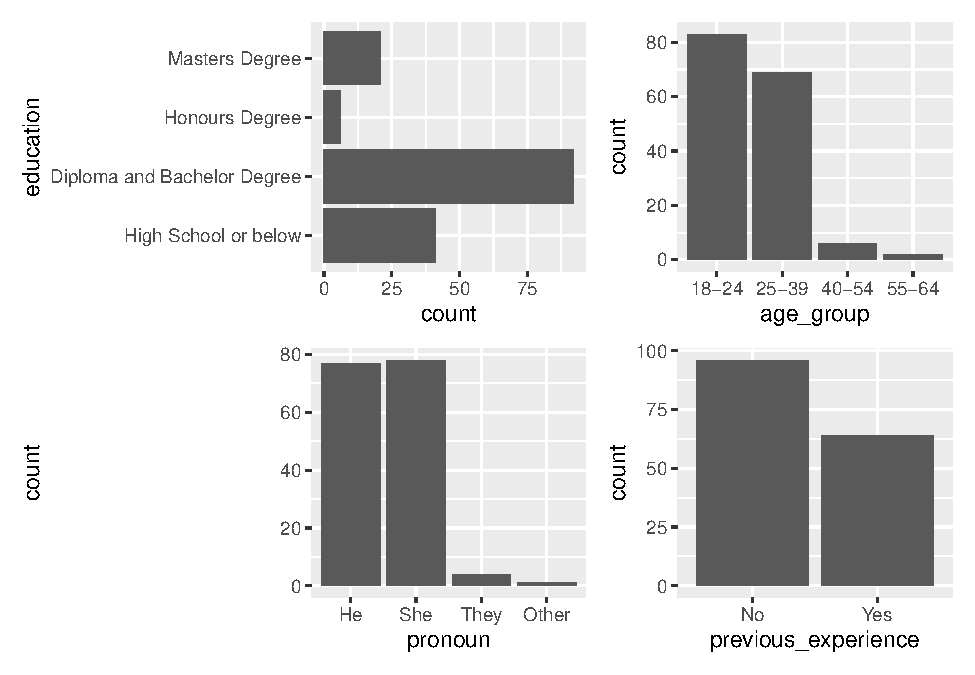
\includegraphics{paper_comparison_files/figure-latex/unnamed-chunk-2-1.pdf}

\hypertarget{data-processing}{%
\section{Data processing}\label{data-processing}}

\hypertarget{results}{%
\section{Results}\label{results}}

\hypertarget{overview-of-the-data}{%
\subsection{Overview of the Data}\label{overview-of-the-data}}

We collected 400 lineup evaluations made by 20 participants in
experiment I and 880 lineup evaluations made by 44 participants in
experiment II. In total, 442 unique lineups were evaluated by 64
subjects. In experiment I, one of the participants skipped all 20
lineups. Hence, the submission was rejected and removed from the
dataset. In experiment II, there was a participant failed one of the two
attention checks, but there was no further evidence of low-effort
throughout the experiment. Therefore, the submission was kept.

\hypertarget{power-comparision}{%
\subsection{Power comparision}\label{power-comparision}}

\begin{enumerate}
\def\labelenumi{\arabic{enumi}.}
\tightlist
\item
  power (visual test vs.~conventional test) (visual test most different
  one (everything test, any departure)) plot figure in a paper, desc,
  exp
\item
  investigate the difference (gap), give examples
\item
  conventional is too sensitive
\item
  make conventional less sensitive (vary alpha)
\end{enumerate}

To model the power of visual test, 10 logistic regression were fit for
different number of evaluations ranged from one to five and two
different types of simulation setting. All 10 models used natural
logarithm of the effect size as the only fixed effect, and whether the
test successfully rejects the null hypothesis as the response variable.
Given the way we define the effect size, it was expected that with
larger effect size, both conventional test and visual test will have
higher probability in rejecting the null hypothesis when it is not true.
The modelling result summarized in \ref{tab:powerglmcubic} and
\ref{tab:powerglmheter} aligned with the expectation as the coefficients
of natural logarithm of the effect size are positive and significant
across all 10 models.

Figure \ref{fig:power-com} illustrates the fitted models, while
providing the local constant estimate of the power of F-test and
Breusch--Pagan test for comparison. Data for the conventional test is
simulated under the model setting described in section \ldots{} and
5000000 samples are drawn for both cubic and heteroskedasticity model.
From Figure \ref{fig:power-com}, it can be observed that the fitted
power of visual test increased as the number of evaluations increased
for both cubic and heteroskedasticity model.

For heteroskedasticity model, this phenomenon was more obvious as the
power of visual tests with evaluations greater than two were always
greater than those with evaluations smaller than two.

For cubic model, the separation between curves was small. The estimated
power of visual tests with three to five evaluations were almost
identical to each other in regards of effect size. In addition, all five
curves peaked at one as effect size increased, suggesting that
identification of non-linearity as a visual task can be completed
reliably by human as long as the departure from null hypothesis is large
enough.

As shown in Figure \ref{fig:power-com}, both F-test and Breusch--Pagan
test generally possessed greater power than visual test. A visual tests
is a collection of test against any alternatives that would create
visual discoverable features, while a conventional test is usually
targeting at a pre-specified alternative. Considering the data
generating process of the model defect was known and controlled in this
research, where all other alternatives have been eliminated except the
one we concerned, the result was suggested that conventional tests were
more sensitive to violations of linearity and homoscedasticity
assumption than visual tests.

It was also found that there was a noticeable gap between curves of the
conventional test and the visual test at around
\(log(\text{effect size}) = 0\) for the cubic model and
\(log(\text{effect size}) = 2.5\) for the heteroskedasticity model,
where the differences in power were greater than 0.6. We further
analysed the lineups with correspoding effect sizes. Figure
\ref{fig:cubic-hard} and \ref{fig:heter-hard} showed that human was
indeed hard to identify the patterns at this level of difficulty. The
visual difference between the true data plot and null plots were almost
unnoticeable.

\hypertarget{effect-of-parameters-on-power-of-the-visual-test}{%
\subsection{Effect of parameters on power of the visual
test}\label{effect-of-parameters-on-power-of-the-visual-test}}

The previous section focuses on the change of effect size relative to
the power of the visual test. However, effect size is only a one
dimensional summarisation of parameters used in data simulation.
Individual factor embedded in the simulation process should also be
analysed.

In cubic model, two major factors that influencing the strength of the
signal are \(a\) and \(b\). Figure \ref{fig:power-com-cubic-a} and
\ref{fig:power-com-cubic-a} illustrates 30 different logistic
regressions fit for different number of evaluations and different number
of observations \(n\). The regressor used in these models was
\(|a|/\sigma\) since the noise level \(\sigma\) needed to be taken into
account. From the figures, we can observe \ldots{}

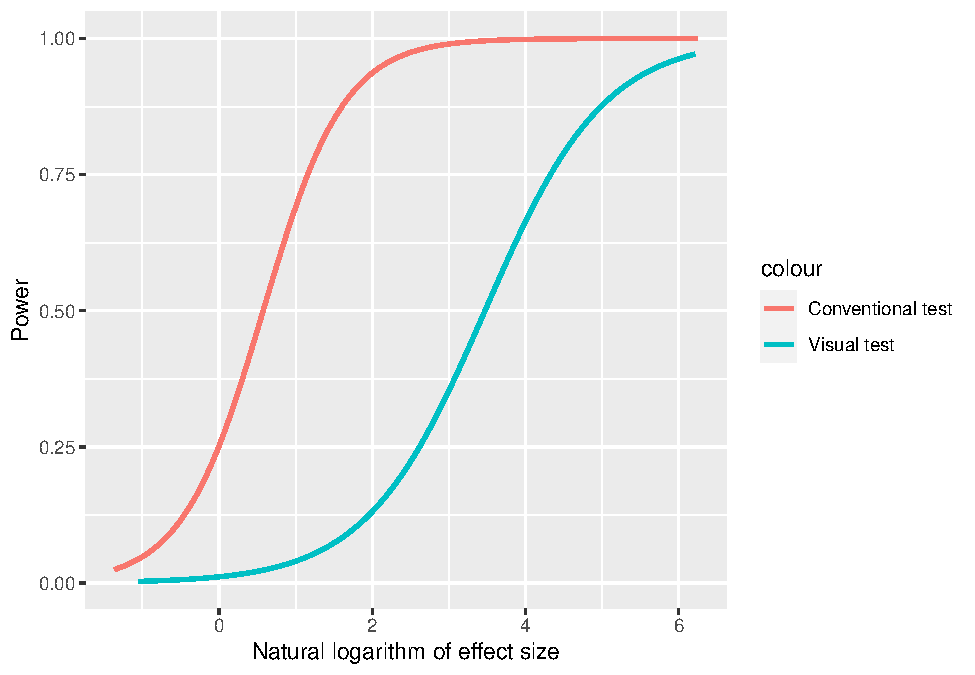
\includegraphics{paper_comparison_files/figure-latex/power-vs-log-effect-size-1.pdf}

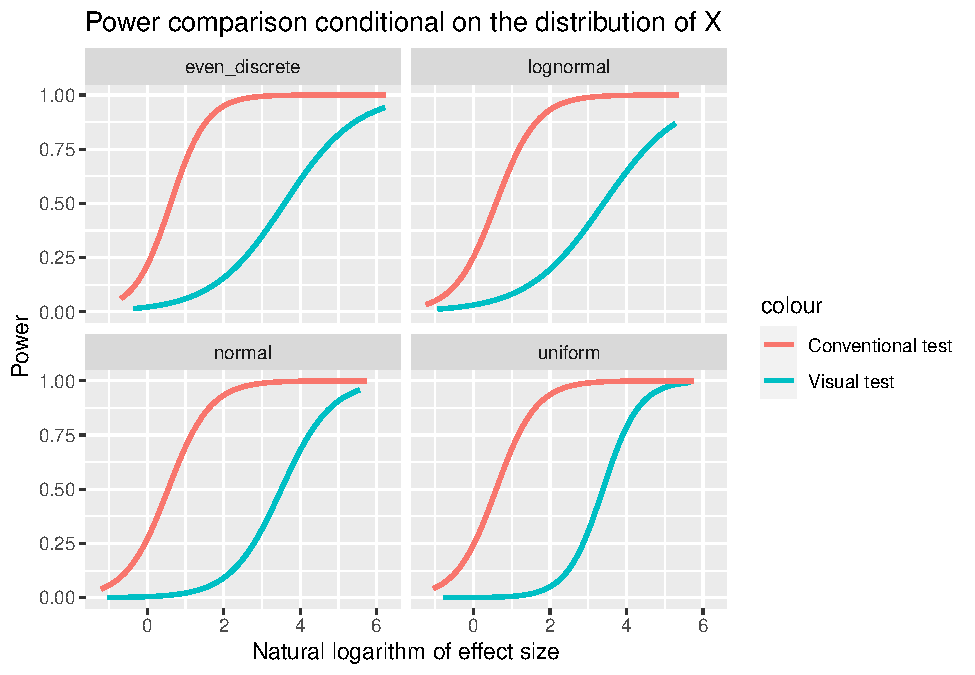
\includegraphics{paper_comparison_files/figure-latex/power-vs-log-effect-size-given-x-dist-1.pdf}

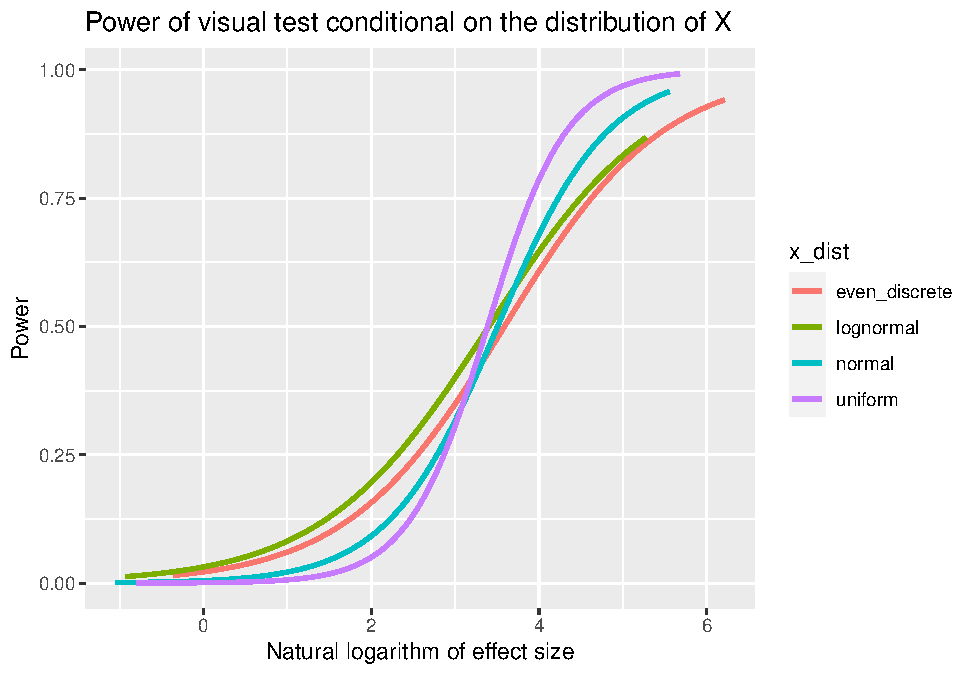
\includegraphics{paper_comparison_files/figure-latex/power-of-visual-test-given-x-dist-1.pdf}

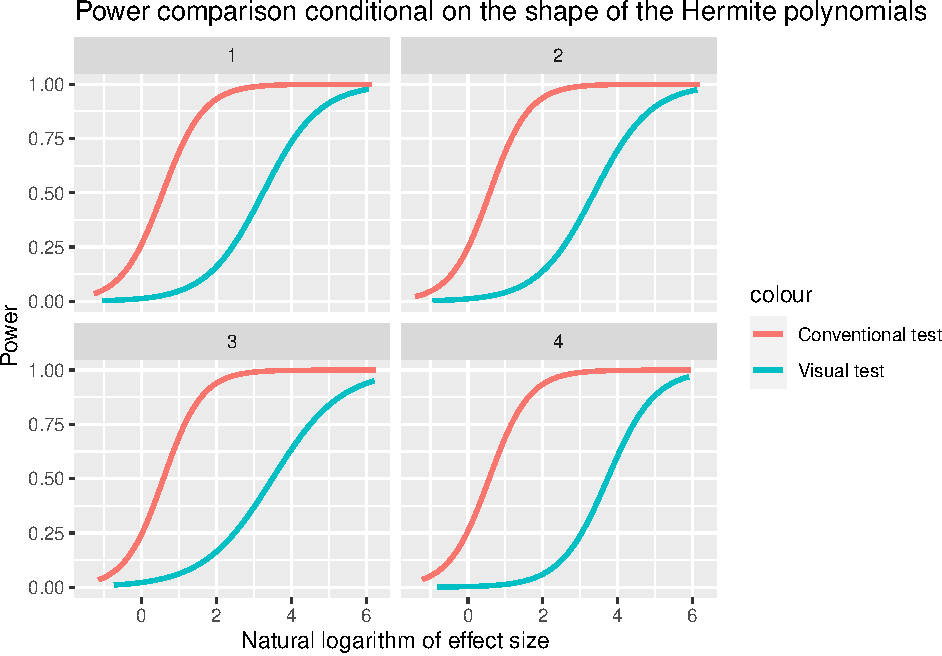
\includegraphics{paper_comparison_files/figure-latex/power-vs-log-effect-size-given-shape-1.pdf}

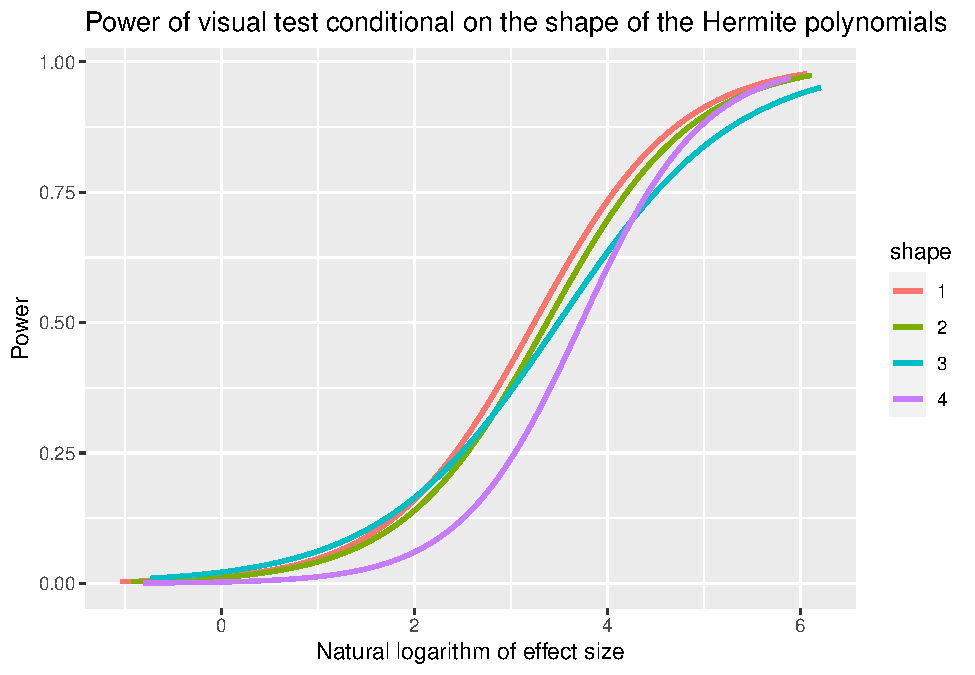
\includegraphics{paper_comparison_files/figure-latex/power-of-visual-test-given-shape-1.pdf}

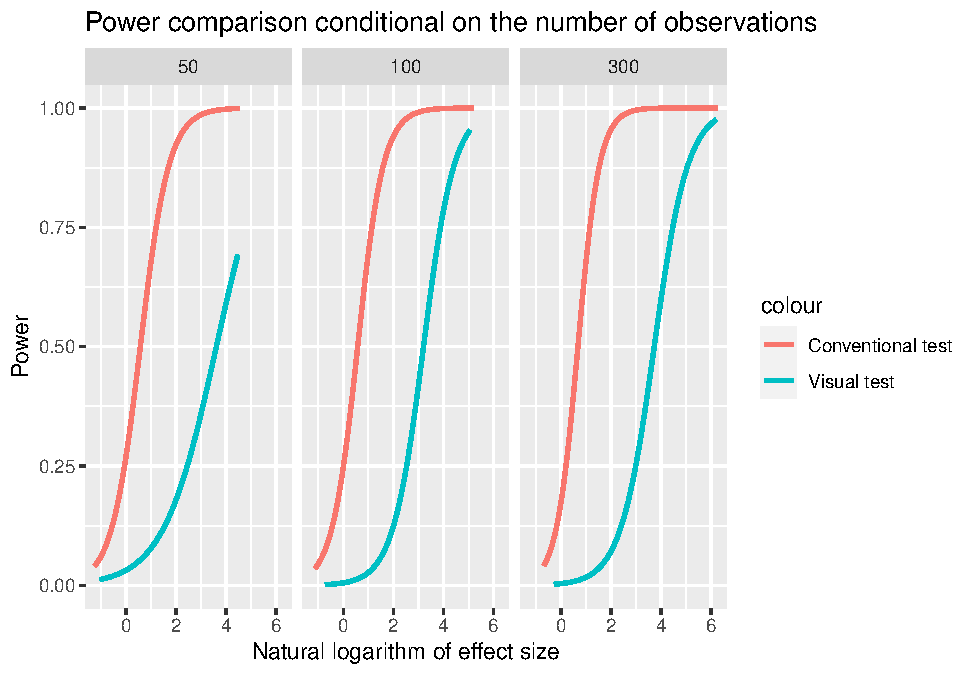
\includegraphics{paper_comparison_files/figure-latex/power-vs-log-effect-size-given-number-of-observations-1.pdf}

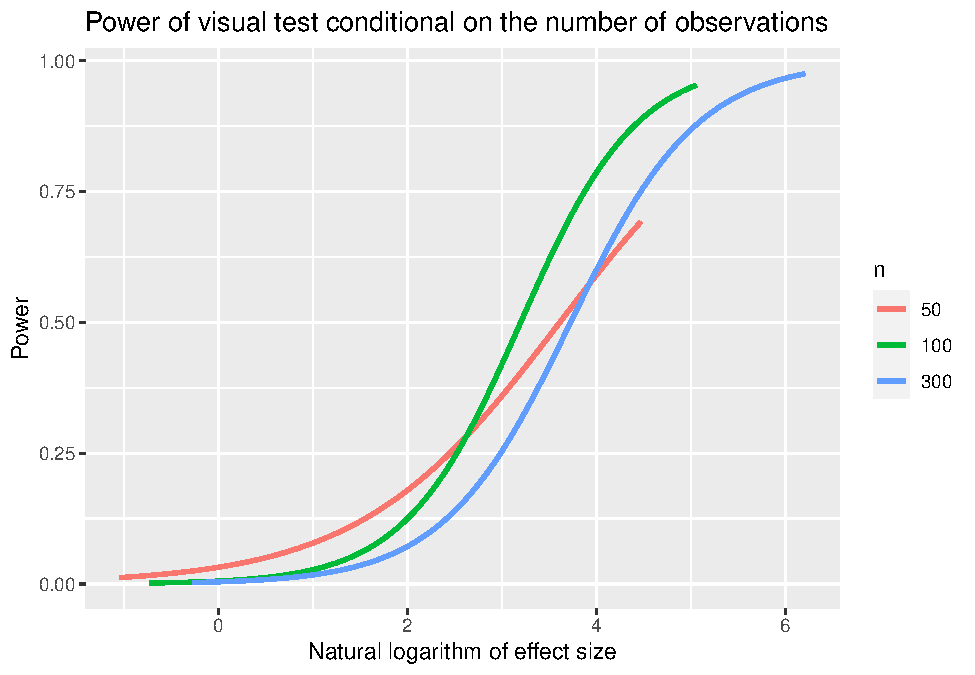
\includegraphics{paper_comparison_files/figure-latex/power-of-visual-test-given-number-of-observations-1.pdf}

\bibliographystyle{tfcad}
\bibliography{paper.bib}




\end{document}
